\chapter{Assessing User's Perceptions of Blockchain}
\label{chap:study}


In this chapter, we present the results of research conducted through an online questionnaire focused on the problem of assessing user's perceptions of blockchain-based technologies. We describe the design that underlies our questionnaire, present the results of the questionnaire and perform an in-depth analysis of those results, in which we explore what trends we are able to infer. Our objectives with this are to assess how users perceive blockchain-based technologies, both in terms of security and complexity, and understand how adoption of such technologies, specifically in our use case, might vary positively, or negatively, comparing to other technologies.

We have highlighted, previously, potential applications of blockchains \cite{pilkington_blockchain_2016, crosby_blockchain_2016, underwood_blockchain_2016}, as well as some research that has already been conducted thus far \cite{biswas_securing_2016, ouaddah_fairaccess:_2017, fotiou_decentralized_2016}. It starts to be clearer that blockchain technology has far more potential, than exclusively as a means to register transactions of decentralized cryptocurrencies. Nonetheless, there's few or nonexistent research in regards as to how humans perceive blockchain technology, much less in our specific use case. Although there's increasing research focused on using blockchain technology, for solving security, privacy and access control issues, such as \cite{maesa_blockchain_2017, ouaddah_access_2017, dorri_blockchain_2017, yue_healthcare_2016}, in an increasingly decentralized and complex society, there's little research over how humans perceive that disruption.

Important factors for the adoption of a given technology, or technique, are the perceived relevance, complexity and suitability for the task at hand: \emph{How can we understand how humans will embrace the blockchain disruption if we don't understand how they perceive the underlying technology?} It is a fact that end-users are increasing their blockchain-based cryptocurrencies adoption \cite{bloomberg_crypto_central} \cite{bloomberg_crypto_altcoins} \cite{nyt_crypto_buble}, along with the market value increase of several cryptocurrencies. Yet, the understanding of how humans embrace these new decentralized applications built on top of blockchains, not only Bitcoin's blockchain but other blockchains as well, is still unknown. This is an enormous gap in our knowledge, in the sense that we have been funding millions of dollars for startups with the promise of building technologies on top of blockchain technologies, yet we cannot even grasp how humans will react to that disruption. If user's perspective is not accounted in the design of new blockchain applications, they would be more likely to fail.

Furthermore, we have yet to understand how users perceive blockchain's complexity or inherent security, if they understand the technology and concepts, or whether such a technology would appeal to them. Do users perceive blockchain as having the same potential as the academic literature suggests? Do users perceive blockchains as solutions to the problems we are, collectively, aiming to solve? These questions are our starting point for the forthcoming statistical study.

The aim of our research is to start filling in that gap by studying how users perceive blockchain-based technology, regarding its security and complexity. This has been done by conducting a statistical study, based on an online questionnaire, that attempts to get insights on these matters. In this study, we focused on two design questions:

\begin{itemize}
	\item \textbf{DQ1} - What is the perceived level of security in blockchain-based solutions, compared to other solutions, specifically centralized solutions?
	\item \textbf{DQ2} - What is the perceived complexity introduced by blockchain-based solutions?
\end{itemize}

The aims of this statistical study are two-fold: \emph{(i)} filling a gap in current knowledge regarding blockchain-based technologies, namely the user perception, and \emph{(ii)} focus on the perceived value of blockchain-based solutions for the challenge of educational certificate issuance, sharing and validation. Specifically, we aim at understanding how users perceive blockchain-based solutions, in the context of educational certificates, in terms of security and complexity. The online questionnaire was conducted with 46 respondents.

\section{Study Design}

In Chapter \ref{chap:related}, we described the importance of educational certificates to validate the achievements and capabilities that a specific individual possesses, to a third-party entity. We also described how, with the growing trend in MOOC-based education, issuing, storing, sharing and validating educational certificates is starting to become and interesting challenge to overcome. Moreover, we have also described how some research has been attempting to solve this challenge by using blockchain technologies. At the same time, we have reviewed how research into security, privacy and access control has been increasingly studying the usage of blockchain technologies to overcome challenges of those fields. With that, we have motivated how a lack of research over human perception of the blockchain technologies can pose further challenges in the adoption and usage of blockchain technologies, in deeper research.

\subsection{Business Actors and Interactions}

An initial set of business actors was established for the processes we described in the questionnaire: \textit{Student}, \textit{Educational Institution} and \textit{Recruiter}. In this situation we are using a third-party actor - \textit{Recruiter} - for a specific use case, of trying to share a digital certificate with a recruiter for the purpose of, for example, validating that a \textit{Student} has the educational background it claims. The \textit{Student} is the requester of the certificate that needs to be issued, or is going to be shared. It is the individual that is the rightful owner of the certificate and should determine who has access to it. The \textit{Educational Institution} is the one that is able to generate new certificates, requested by the Requester. It has the capability to validate all requests as well as issue the certificates. Finally, the \textit{Recruiter} serves the purpose of being an individual, with which a certificate might be shared and might want to validate its authenticity.

\begin{figure}[htb]
	\centering
	\begin{subfigure}[b]{0.3\textwidth}
		\centering
		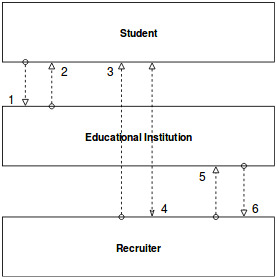
\includegraphics[width=0.8\textwidth]{Scenario1}
		\caption{Interactions in Scenario 1}
		\label{fig: Scenario1}
	\end{subfigure}
	%
	\begin{subfigure}[b]{0.3\textwidth}
		\centering
		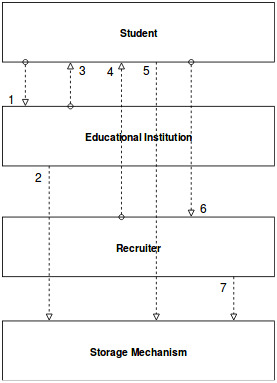
\includegraphics[width=0.8\textwidth]{Scenario2}
		\caption{Interactions in Scenario 2}
		\label{fig: Scenario2}
	\end{subfigure}
	%
	\begin{subfigure}[b]{0.3\textwidth}
		\centering
		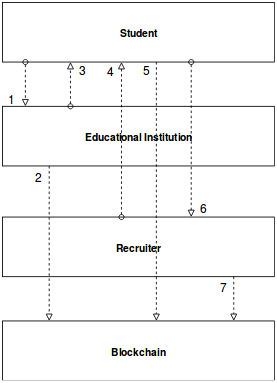
\includegraphics[width=0.8\textwidth]{Scenario3}
		\caption{Interactions in Scenario 3}
		\label{fig: Scenario3}
	\end{subfigure}

	\caption{Interactions presented to Respondents.}
\end{figure}

We used these actors as the basis to develop more complex scenarios and interactions, which we then used in our questionnaire. Respondents were presented with 3 interactions between these actors, as \gls{bpmn} \cite{BPMN} models, presented, respectively in Figure \ref{fig: Scenario1}, Figure \ref{fig: Scenario2} and Figure \ref{fig: Scenario3}. The context in which these interactions were presented is explained, in detail, in the forthcoming section. The three scenarios the respondents had to analyze described:
\emph{(i)} a typical scenario of issuing, sharing and validating an educational certificate, \emph{(ii)} a typical scenario, using an undisclosed storage mechanism, such as a database, with added access control functionality, and \emph{(iii)} a typical scenario, using a blockchain, with added access control functionality.



\subsection{Methodology}

This section discusses the methodology, used throughout the questionnaire, specifically the design of the questionnaire and its contents, and afterwards, the presentation and distribution methods are explained.

\subsubsection{Questionnaire Layout}

The questionnaire was designed to target professionals in multiple industries with different backgrounds and knowledge levels. It had 28 questions, of which 21 were mandatory questions and 7 were optional. There were 5 sections on the questionnaire: \textit{Introduction}, \textit{Background}, \textit{Exercise 1}, \textit{Exercise 2} and \textit{Final Survey}. There was no time limit nor were the respondents' participation offered any incentives. Participation was completely voluntary.

\subsubsection{Section Detail and Questions}

\textit{Introduction} explained the research objectives, the context in which it was inserted and it stated that all answers were anonymous and would only be used, and shared, for academic purposes.
%
\textit{Background} had four questions, with the aim of assessing respondents' professional and academic background, as well as their perceived knowledge of specific technologies and concepts. Those questions were:

\begin{enumerate}
	\item Do you have any academic or professional background related with Information Security?
	\item Which industry best fits with your professional experience?
	\item Which professional role best fits your experience?
	\item How do you classify your knowledge of the following concepts?
\end{enumerate}

In \textit{Exercise 1} and \textit{Exercise 2}, respondents were asked to answer specific questions. In \textit{Exercise 1} there were two separate scenarios to analyze. In \textit{Exercise 2} there was only one scenario to analyze. In each scenario, there was a simple \gls{bpmn} \cite{BPMN} model followed by a description of the interactions between the actors. All three scenarios had exactly the same 7 questions:

\begin{enumerate}
	\item Which level of security do you perceive in each interaction?
	\item Which level of security do you perceive in the entire process?
	\item What could make it more secure?
	\item Select any interactions you perceive as allowing unauthorized access to information being shared.
	\item If you were a Student, what would be your willingness to share information, in this context, with a Recruiter?
	\item  If you were a Student, what would be your confidence that the information you share is secure and no one, except the Recruiter, will access it?
	\item Which level of complexity do you perceive in each interaction?
\end{enumerate}

In the last section, \textit{Final Survey}, the respondents were asked two additional questions and a placeholder for some comments, if necessary:

\begin{enumerate}
	\item Do you think any of the previous 3 scenarios was more secure than the others?
	\item Do you believe knowledge of Information Security, its applications and concepts, is at an adequate level in your professional environment?
\end{enumerate}

Out of the 7 questions, in \textit{Exercise 1} and in \textit{Exercise 2}, 5 were based on Likert scales from 0 to 4, where 0 was the lowest possible value and 4 was the highest possible value. 1 question was an open-ended question - and 1 was a checkbox question. These questions, from each scenario - 21 questions in total - were the core of our study.The respondents were never asked to compare any scenario, but only asked to answer the same questions for each scenario.

\subsubsection{Distribution Methods}

Two versions were made out of the same questionnaire. The first version had the following sequence: Typical scenario $\,\to\,$ Storage Mechanism scenario $\,\to\,$ Blockchain scenario. The second version had the following sequence: Storage Mechanism scenario $\,\to\,$ Typical scenario $\,\to\,$ Blockchain scenario. The questionnaire was made available online at a specific URL \footnote{https://hugomartins.io/human-perception-infosec/} and, upon clicking on it, respondents were redirected to one of the versions without knowing which version and without knowing that several versions existed. The aim of this separation was to try and mitigate the learning effect bias that might arise when analyzing results of a questionnaire answered on a given sequence

The questionnaire was pretested with 1 respondent to validate there were no problems, before distribution and, after necessary corrections, was distributed. Distribution took place, initially, over email to a controlled group of 5 people to ensure the randomization system was working properly and that no errors occurred with submission, this was in order mitigate further problems before sending the questionnaire to more people. After that, it was sent, via email, to a group of 50 people, mainly professionals. That group grew to approximately 150 people. After that, the questionnaire was also posted on HackerNews \footnote{https://news.ycombinator.com/item?id=17064032}, as a LinkedIn post \footnote{https://www.linkedin.com/feed/update/urn:li:activity:6401809377023533056} and in Reddit: in /r/Assistance \footnote{https://www.reddit.com/r/Assistance/comments/8jk3hf/human\_perception\_of\_information\_security\_for} and /r/SampleSize  \footnote{https://www.reddit.com/r/SampleSize/comments/8jk5ej/academic\_human\_perception\_of\_information\_security}. The questionnaire was open for submission from May 9, 2018, until May 20, 2018. Overall, we were able to reach 82 views, of which 46 answered the questionnaire completely.

\section{Results}


This section presents the results of the questionnaire. We have analyzed both versions of the questionnaire separately, \textit{Version 1} and \textit{Version 2}, and performed a combined analysis, with both versions' data sets. This helps when discussion what it is possible to conclude from the results by taking into account possible learning effects' bias, as well as define the limitations that can be overcome in future work, discussed in Chapter \ref{chap:conclusion}.

This section is structured in direct relation to the design questions outlined, in the beginning of this chapter, by looking at the data that relates to each of them.

As described previously, 46 respondents answered the questionnaire, with 24 respondents answering \textit{Version 1} (52\%) and 22 respondents answering \textit{Version 2} (48\%). There was a balance between respondents with backgrounds related to Information Security - with 52\% of the respondents saying they do have a background related to Information Security. Nonetheless, in \textit{Version 1}, 62.5\% of the respondents said they did not have a background related to Information Security. Industries and Roles (see Table \ref{tab: industry} and Table \ref{tab: roles}) tended to be in the area of Software Development.

For simplicity of our analysis, we have corrected the switch made between \textit{Version 1} and \textit{Version 2}, when reporting the results, in order to allow a direct comparison between both data sets, instead of having to mentally compare them, using the sequence used in Version 1.

\begin{table}[htb]
	\centering
	\caption{Industry Frequency}
	\label{tab: industry}
	\begin{tabular}{l|cc|c}
		\hline \bf Industry & \bf Version 1 & \bf Version 2 & \bf Both \\ \hline
		Consultancy         & 5             & 1             & 6        \\
		Telecom.            & 1             & 1             & 2        \\
		Software Dev.       & 9             & 15            & 24       \\
		R\&D                & 1             & 1             & 2        \\
		Academic            & 4             & 3             & 7        \\
		Other               & 2             & 1             & 3        \\
		N.A.                & 1             & 0             & 1        \\
		Health              & 1             & 0             & 1        \\
		\hline
	\end{tabular}
\end{table}

\begin{table}[htb]
	\centering
	\caption{Role Frequency}
	\label{tab: roles}
	\begin{tabular}{l|cc|c}
		\hline \bf Role  & \bf Version 1 & \bf Version 2 & \bf Both \\ \hline
		Software Dev.    & 13            & 12            & 25       \\
		Researcher       & 2             & 2             & 4        \\
		Professor        & 1             & 15            & 24       \\
		Business Manager & 5             & 1             & 6        \\
		Project Manager  & 1             & 4             & 5        \\
		Other            & 1             & 1             & 2        \\
		N.A.             & 1             & 0             & 1        \\
		\hline
	\end{tabular}
\end{table}

Respondent's perceived knowledge of specific concepts, from 0 (lowest) to 4 (highest), slightly varied between versions, with \textit{Version 2} presenting a more knowledgeable set of respondents, in most concepts (see Table \ref{tab: knowledge}), with the concepts being: \emph{(i)} Access Control; \emph{(ii)} Encryption; \emph{(iiii)} blockchain; \emph{(iv)} Data Integrity; \emph{(v)} Malware; \emph{(vi)} Phishing; \emph{(vii)} Data Confidentiality; \emph{(viii)} \gls{bpmn}; \emph{(ix)} Data Storage; \emph{(x)} Unauthorized Access.

\begin{table}[htb]
	\centering
	\caption{Reported Knowledge Using the Scale 0 (Lowest) to 4 (Highest)}
	\label{tab: knowledge}
	\begin{tabular}{c|cccc|cc}
		\hline
		\bf Concept & \multicolumn{2}{c}{\bf Version 1} & \multicolumn{2}{c}{\bf Version 2} \vrule & \multicolumn{2}{c}{\bf Both}                                             \\
		\hline
		            & $\tilde{x}$                       & $\sigma_{x}$                             & $\tilde{x}$                  & $\sigma_{x}$ & $\tilde{x}$ & $\sigma_{x}$ \\
		\hline
		1           & 1.92                              & 0.97                                     & 2.36                         & 1.18         & 2.13        & 1.09         \\
		2           & 1.67                              & 1.05                                     & 2.14                         & 1.13         & 1.89        & 1.10         \\
		3           & 1.33                              & 0.87                                     & 1.05                         & 0.84         & 1.20        & 0.86         \\
		4           & 1.83                              & 1.09                                     & 2.14                         & 1.21         & 1.98        & 1.15         \\
		5           & 1.71                              & 0.91                                     & 1.82                         & 0.96         & 1.76        & 0.92         \\
		6           & 1.96                              & 0.91                                     & 2.14                         & 0.94         & 2.04        & 0.92         \\
		7           & 2.46                              & 1.02                                     & 2.46                         & 1.01         & 2.46        & 1.01         \\
		8           & 0.83                              & 1.01                                     & 1.36                         & 1.36         & 1.09        & 1.21         \\
		9           & 2.29                              & 1.00                                     & 2.36                         & 1.33         & 2.32        & 1.16         \\
		10          & 2.00                              & 1.02                                     & 2.09                         & 1.27         & 2.04        & 1.13         \\
		\hline
	\end{tabular}
\end{table}

Regarding our background results, we can conclude that our sample tends towards Software Development, followed by professionals from Academia. This means that our sample is potentially more knowledgeable to having more knowledge on general technology topics, than a more mixed sample would. \textit{Version 1} respondents reported a below-average knowledge of the presented concepts, with a lower standard deviation, while \textit{Version 2} respondents reported a higher than average knowledge of the presented concepts, with a less concentrated set of answers. All coefficients of variation, in the compound analysis, are lower than 1 (between \textit{cv = 0.41} and \textit{cv = 0.72}), except for \gls{bpmn} (\textit{cv = 1.11}). The same happens for each separate version, with different boundaries.

\subsection{DQ1}

\begin{quote}
	\textit{What is the perceived level of security in blockchain-based solutions, compared to other solutions?}
\end{quote}

To answer this question, we took special attention to questions 1, 2 and 4 of each of the scenarios. In questions 1 and 2, respondents were asked to evaluate the perceived security of a given scenario. The evaluations were for the process in its entirety and for each interaction in the scenario. Question 4 asked respondents to select the interactions they perceived as allowing unauthorized questions. We have also taken in consideration the answers given in the final question, in which respondents were forced to choose which scenario was the most secure.

Starting from the last question, an overwhelming majority of the respondents answered that they perceived the scenario using blockchain to be the most secure (see Table \ref{tab: mostSecure}) - when forced to choose.

\begin{table}[htb]
	\centering
	\caption{Most Secure Scenario (Total Amount of Responses)}
	\label{tab: mostSecure}
	\begin{tabular}{l|ccc}
		\hline \bf Answer & \bf Version 1 & \bf Version 2 & \bf Both \\ \hline
		None              & 1             & 1             & 2        \\
		Scenario 1        & 1             & 4             & 5        \\
		Scenario 2        & 3             & 3             & 6        \\
		Scenario 3        & 19            & 14            & 33       \\
		\hline
	\end{tabular}
\end{table}

This suggests that there's a tendency to believe that blockchain-based solutions are perceived as being more secure than other solutions. The fact that users were forced to choose one or none of the scenarios makes it more clear that, although we cannot claim any justification for it, respondents had a tendency to claim that blockchain-based solutions are more secure than other solutions. Even more interesting is that not only did respondents choose blockchain-based solutions against the typical scenario but the same occurred for the scenario that used a basic Storage Mechanism, instead of the blockchain-based one.

For the first question, which asked for the perceived level of security in each scenario (see Table \ref{tab: perceivedSecurity}), we witness similar results. We witness the same effect, in \textit{Version 2}, as we had previously, although the data is more spread (\textit{$\sigma_{x}$ = 1.23}).

\begin{table}[htb]
	\centering
	\caption{Perceived Security / Scenario Using the Scale 0 (Lowest) to 4 (Highest)}
	\label{tab: perceivedSecurity}
	\begin{tabular}{c|cccc|cc}
		\hline
		Scenario & \multicolumn{2}{c}{\bf Version 1} & \multicolumn{2}{c}{\bf Version 2} \vrule & \multicolumn{2}{c}{\bf Both}                                             \\
		\hline
		         & $\tilde{x}$                       & $\sigma_{x}$                             & $\tilde{x}$                  & $\sigma_{x}$ & $\tilde{x}$ & $\sigma_{x}$ \\
		\hline
		1        & 2.13                              & 0.99                                     & 2.50                         & 1.23         & 2.30        & 1.11         \\
		2        & 2.83                              & 0.96                                     & 2.36                         & 0.95         & 2.61        & 0.98         \\
		3        & 3.00                              & 0.89                                     & 2.91                         & 0.87         & 2.96        & 0.87         \\
		\hline
	\end{tabular}
\end{table}

We can understand, by studying the coefficients of variation (Version 1: Scenario 1 (\textit{cv = 0.47}), Scenario 2 (\textit{cv = 0.34}), Scenario 3 (\textit{cv = 0.29}); Version 2: Scenario 1 (\textit{cv = 0.48}), Scenario 2 (\textit{cv = 0.40}), Scenario 3 (\textit{cv = 0.30}) that respondents' answers became more concentrated when it comes to blockchain-based solutions (Scenario 3), while being more dispersed in Storage Mechanism (Scenario 2) and even more in the typical process (Scenario 1). This further reinforces the appearing tendency.

By studying the results of the evaluation by interaction, in each scenario, and with the scenario as a whole, the data is less clear than previous answers. Results, seen in Table \ref{tab: perceivedInteractionSecurity}, have shown an increase in the dispersion of the data which impacts mean-based analysis. It is interesting that, contrary to what had happened when asked about the security of the entire process, in this case, in \textit{Version 1}, we cannot see a major difference between the results of Scenario 2 and Scenario 3. Nonetheless, we still see the same patterns as in the previous results, in \textit{Version 2} and when considering the data sets combined.

\begin{table}[htb]
	\centering
	\caption{Perceived Interaction Security / Scenario Using the Scale 0 (Lowest) to 4 (Highest)}
	\label{tab: perceivedInteractionSecurity}
	\begin{tabular}{c|cccc|cc}
		\hline
		Scenario & \multicolumn{2}{c}{\bf Version 1} & \multicolumn{2}{c}{\bf Version 2} \vrule & \multicolumn{2}{c}{\bf Both}                                             \\
		\hline
		         & $\tilde{x}$                       & $\sigma_{x}$                             & $\tilde{x}$                  & $\sigma_{x}$ & $\tilde{x}$ & $\sigma_{x}$ \\
		\hline
		1        & 2.26                              & 1.30                                     & 2.58                         & 1.21         & 2.42        & 1.26         \\
		2        & 2.71                              & 1.13                                     & 2.27                         & 1.43         & 2.50        & 1.30         \\
		3        & 2.68                              & 1.12                                     & 2.72                         & 1.19         & 2.70        & 1.15         \\
		\hline
	\end{tabular}
\end{table}

In Figure \ref{fig: perceivedInteractionSecurityOne} we expose the data used to generate Table \ref{tab: perceivedInteractionSecurity}'s \textit{Version 1}, as line charts, in which the data sets for each scenario have been run through a probability density function. This allows us to see that the mean, for Scenario 2, is highly influenced by more skewed distributions and, at the same time, it confirms, visually, the data about the process as a whole. Scenario 3 is visually more secure and concentrated - the interactions perceived as more secure, individually.

\begin{figure}[htb]
	\centering
	\begin{subfigure}[b]{0.49\textwidth}
		\centering
		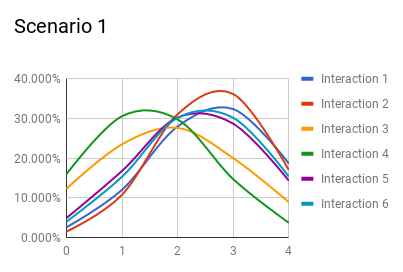
\includegraphics[width=\linewidth]{V1-S1-Security.png}
	\end{subfigure}
	%
	\begin{subfigure}[b]{0.49\textwidth}
		\centering
		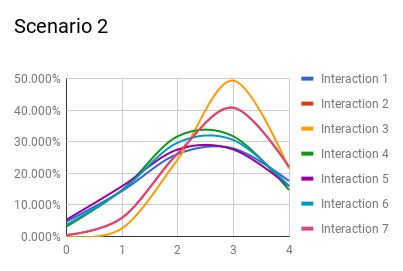
\includegraphics[width=\linewidth]{V1-S2-Security.png}
	\end{subfigure}
	%
	\hfill
	\begin{subfigure}[b]{0.49\textwidth}
		\centering
		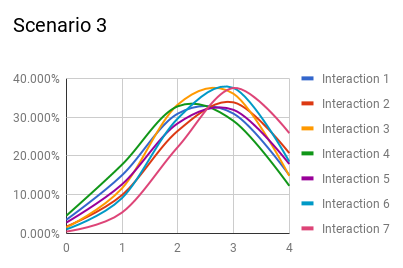
\includegraphics[width=\linewidth]{V1-S3-Security.png}
	\end{subfigure}

	\caption{Probability Density of Perceived Interaction Security (Version 1)}
	\label{fig: perceivedInteractionSecurityOne}
\end{figure}

At the same time, in Figure \ref{fig: perceivedInteractionSecurityTwo} we expose the data used to generate Table \ref{tab: perceivedInteractionSecurity}'s \textit{Version 2}. The visualizations closely resembles the one presented in Figure \ref{fig: perceivedInteractionSecurityOne}. This is relevant due to the fact that the aggregate numbers, shown in Table \ref{tab: perceivedInteractionSecurity}, only allow us to have a high-level understanding, of the respondents' perception. The visualizations help understand that, even in more detail, the data is similarly distributed, although, somehow skewed to the left, in Scenario 1, and skewed to the right.

\begin{figure}[htb]
	\centering
	\begin{subfigure}[b]{0.49\textwidth}
		\centering
		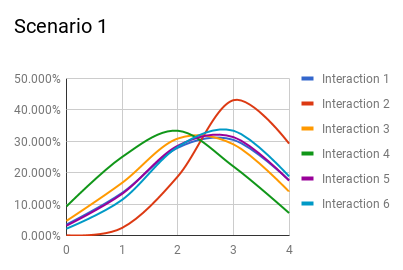
\includegraphics[width=\linewidth]{V2-S1-Security.png}
	\end{subfigure}
	%
	\begin{subfigure}[b]{0.49\textwidth}
		\centering
		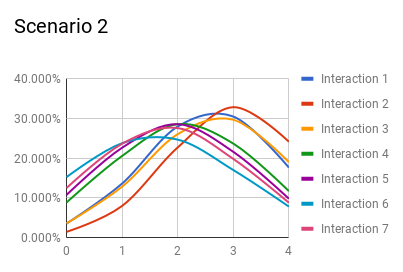
\includegraphics[width=\linewidth]{V2-S2-Security.png}
	\end{subfigure}
	%
	\hfill
	\begin{subfigure}[b]{0.49\textwidth}
		\centering
		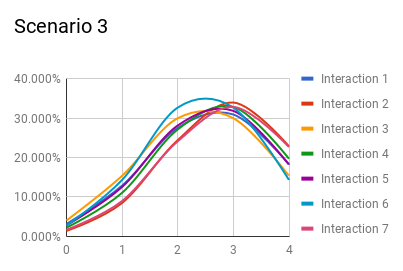
\includegraphics[width=\linewidth]{V2-S3-Security.png}
	\end{subfigure}

	\caption{Probability Density of Perceived Interaction Security (Version 2)}
	\label{fig: perceivedInteractionSecurityTwo}
\end{figure}

Finally, respondents also perceived that sharing the certificate, under a blockchain-based solution, had fewer interactions with the possibility of allowing unauthorized access to data, than with the typical purpose. The same is true for blockchain-based solutions over the Storage Mechanism.

\subsection{DQ2}

\begin{quote}
	\textit{What is the perceived complexity introduced by blockchain-based solutions?}
\end{quote}

\begin{table}[htb]
	\centering
	\caption{Perceived Complexity / Scenario Using the Scale 0 (Lowest) to 4 (Highest)}
	\label{tab: perceivedComplexity}
	\begin{tabular}{c|cccc|cc}
		\hline
		Scenario & \multicolumn{2}{c}{\bf Version 1} & \multicolumn{2}{c}{\bf Version 2} \vrule & \multicolumn{2}{c}{\bf Both}                                             \\
		\hline
		         & $\tilde{x}$                       & $\sigma_{x}$                             & $\tilde{x}$                  & $\sigma_{x}$ & $\tilde{x}$ & $\sigma_{x}$ \\
		\hline
		1        & 1.56                              & 1.51                                     & 1.47                         & 1.13         & 1.51        & 1.14         \\
		2        & 1.96                              & 1.21                                     & 1.71                         & 1.25         & 1.82        & 1.23         \\
		3        & 2.25                              & 1.26                                     & 1.97                         & 2.00         & 2.12        & 1.24         \\
		\hline
	\end{tabular}
\end{table}

For this question, we have analyzed the answers to question 7 of each scenario, which asked respondents to grade each interaction they were shown, in terms of its complexity. We present the mean for all interactions' evaluation and also the standard deviation, per scenario (see Table \ref{tab: perceivedSecurity}). The results show that there's an increase in the perceived complexity of blockchain-based solutions. In this case, contrary to what happened with the previous design question, we do not see a pronounced learning bias as, regardless of the order of the questions, the tendency remained the same - and the compound analysis reflected that situation. It is also interesting to notice that, when asked about the concept of complexity, the dispersion of data increases, specially when compared to the concept of security.

\begin{figure}[htb]
	\centering
	\begin{subfigure}[b]{0.49\textwidth}
		\centering
		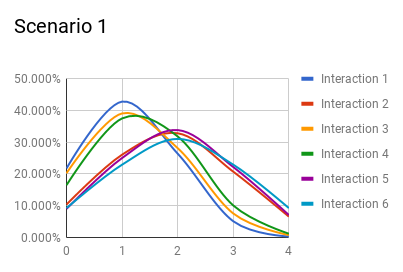
\includegraphics[width=\linewidth]{V1-S1-Complexity.png}
	\end{subfigure}
	%
	\begin{subfigure}[b]{0.49\textwidth}
		\centering
		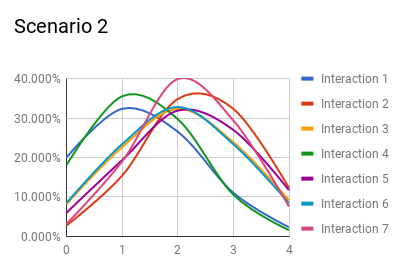
\includegraphics[width=\linewidth]{V1-S2-Complexity.png}
	\end{subfigure}
	%
	\hfill
	\begin{subfigure}[b]{0.49\textwidth}
		\centering
		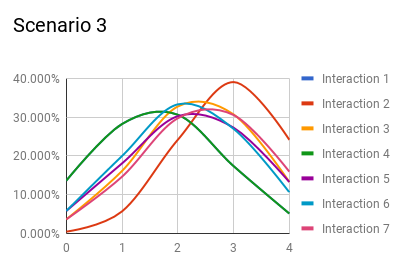
\includegraphics[width=\linewidth]{V1-S3-Complexity.png}
	\end{subfigure}

	\caption{Probability Density of Perceived Interaction Complexity (Version 1)}
	\label{fig: perceivedInteractionComplexityOne}
\end{figure}

\begin{figure}[htb]
	\centering
	\begin{subfigure}[b]{0.49\textwidth}
		\centering
		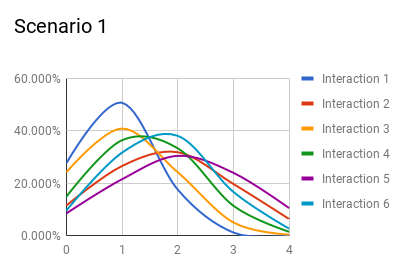
\includegraphics[width=\linewidth]{V2-S1-Complexity.png}
	\end{subfigure}
	%
	\begin{subfigure}[b]{0.49\textwidth}
		\centering
		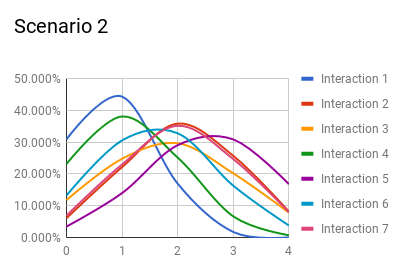
\includegraphics[width=\linewidth]{V2-S2-Complexity.png}
	\end{subfigure}
	%
	\hfill
	\begin{subfigure}[b]{0.49\textwidth}
		\centering
		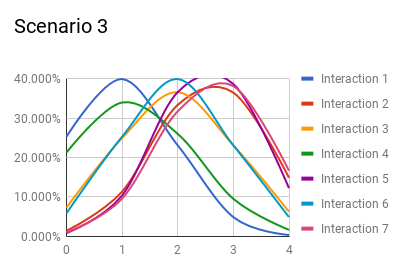
\includegraphics[width=\linewidth]{V2-S3-Complexity.png}
	\end{subfigure}

	\caption{Probability Density of Perceived Interaction Complexity (Version 2)}
	\label{fig: perceivedInteractionComplexityTwo}
\end{figure}

Figure \ref{fig: perceivedInteractionComplexityOne} and Figure \ref{fig: perceivedInteractionComplexityTwo} allow us to perform the same visual comparison, such as in the previous section. What we see indicates what has been shown in the high-level picture, both in terms of mean and standard deviation. For example, in the blockchain-based solutions (Scenario 3), in \textit{Version 2} , the data is very spread when compared inter-interaction but it seems to be much more concentrated for each interaction than in \textit{Version 1}.

\section{Summary}

This study presents an overlap between several areas of research: Information Security, Blockchain, Educational Certificates and Human Perception. We sought to explore how those interact by conducting an online questionnaire followed by a study that would shed some light over how humans perceive blockchain technology, in terms of security and complexity, in an Educational Certificate use case. The results have indicated a tendency for users to perceive blockchain technology as more secure but, alas, more complex too - at least in this particular domain. This research is a starting point to better understand how humans perceive blockchain technology.